\documentclass[10pt,twocolumn,letterpaper]{article}

\usepackage{cvpr}
\usepackage{times}
\usepackage{epsfig}
\usepackage{graphicx}
\usepackage{amsmath}
\usepackage{amssymb}

% Include other packages here, before hyperref.

% If you comment hyperref and then uncomment it, you should delete
% egpaper.aux before re-running latex.  (Or just hit 'q' on the first latex
% run, let it finish, and you should be clear).
\usepackage[pagebackref=true,breaklinks=true,letterpaper=true,colorlinks,bookmarks=false]{hyperref}

% \cvprfinalcopy % *** Uncomment this line for the final submission

\def\cvprPaperID{****} % *** Enter the CVPR Paper ID here
\def\httilde{\mbox{\tt\raisebox{-.5ex}{\symbol{126}}}}

% Pages are numbered in submission mode, and unnumbered in camera-ready
\ifcvprfinal\pagestyle{empty}\fi
\begin{document}

%%%%%%%%% TITLE
\title{\LaTeX\ Author Guidelines for CVPR Proceedings}

\author{First Author\\
Institution1\\
Institution1 address\\
{\tt\small firstauthor@i1.org}
% For a paper whose authors are all at the same institution,
% omit the following lines up until the closing ``}''.
% Additional authors and addresses can be added with ``\and'',
% just like the second author.
% To save space, use either the email address or home page, not both
\and
Second Author\\
Institution2\\
First line of institution2 address\\
{\tt\small secondauthor@i2.org}
}

\maketitle
%\thispagestyle{empty}

\maketitle
%\thispagestyle{empty}

%%%%%%%%% ABSTRACT
\begin{abstract}
   pass
\end{abstract}

%%%%%%%%% BODY TEXT
\section{Introduction}

\textbf{The importance of our research area} \\

\textbf{Some progress in sketch based image retrieval} \\

\textbf{Difficulty in Zero-shot setup and some possible solutions} \\

\textbf{Our proposed methods and their advantages} \\

\textbf{itemize our contributions in this paper} \\




%\begin{figure}[t]
%\begin{center}
%\fbox{\rule{0pt}{2in} \rule{0.9\linewidth}{0pt}}
   %\includegraphics[width=0.8\linewidth]{egfigure.eps}
%\end{center}
%   \caption{Example of caption.  It is set in Roman so that mathematics
%   (always set in Roman: $B \sin A = A \sin B$) may be included without an
%   ugly clash.}
%\label{fig:long}
%\label{fig:onecol}
%\end{figure}




%\begin{figure*}
%\begin{center}
%\fbox{\rule{0pt}{2in} \rule{.9\linewidth}{0pt}}
%\end{center}
%   \caption{Example of a short caption, which should be centered.}
%\label{fig:short}
%\end{figure*}

\section{Related Work}

\subsection{Sketch-based image retrieval}

\subsection{Zero-Shot Learning}

\subsection{Cross-modal domain translation}


\begin{figure*}
\begin{center}
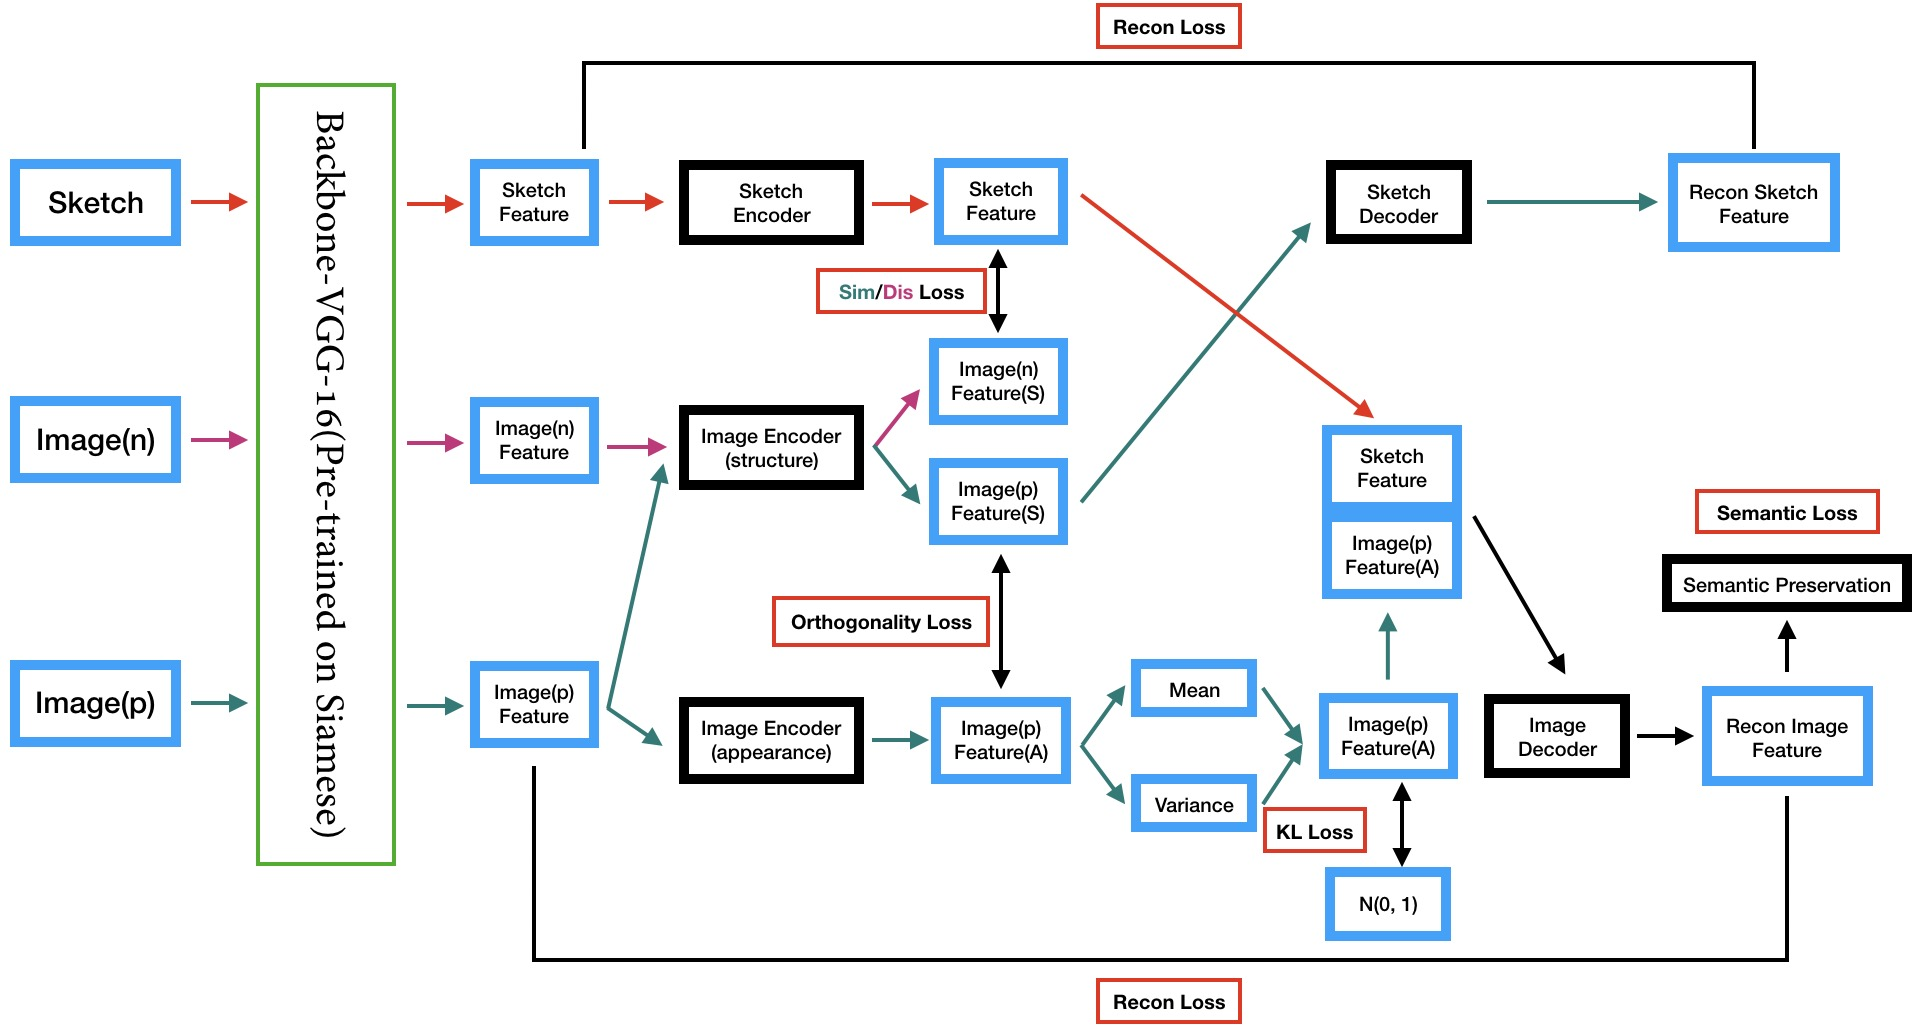
\includegraphics[width=0.95\linewidth]{model_structure.jpg}
\end{center}
   \caption{Model Structure}
\label{fig:short}
\end{figure*}

\section{Methodology}
There will be five parts in this section. 
Sec. \ref{3.1} defines the our targeted problem and briefly introduce our framework. 
Sec. \ref{3.2} introduce the feature extractor. 
Sec. \ref{3.3} introduce the parallel VAEs. 
Sec. \ref{3.4} introduce the semantic preservation module. 
Sec. \ref{3.5} introduce the design of loss functions during training procedure.

\subsection{Problem Definition} \label{3.1}
In this paper, we focus on solving the problem of hand-free sketch-based image retrieval under zero-shot setup, where only the sketches and images from seen class are used during training stage. 
Our proposed framework is expected to use the sketches to retrieve the images, the categories of which have never appeared during training.

We first provide a definition of the SBIR in zero-shot setting. 
Given a dataset $S=\{(x_i^{img}, x_i^{ske}, x_i^{sem}, y_i)|y_i \in \mathcal{Y}\}$, where $x_i^{img}$, $x_i^{ske}$, $x_i^{sem}$ and $y_i$ are corresponding to the image, sketch, semantic representation and class label. 
Following the zero-shot setting in \cite{yelamarthi2018zero}, we split all classes $\mathcal{Y}$ into $\mathcal{Y}_{train}$ and $\mathcal{Y}_{test}$ according to whether the label exists in ImageNet\cite{deng2009imagenet}, where no overlap exists between two label set, i.e. $\mathcal{Y}_{train} \cap \mathcal{Y}_{test} = \emptyset$. 
Based on the partition of label set $\mathcal{Y}$, we split dataset into $S_{train}$ and $S_{test}$. 
Our model need to disentangle structure representations of image using data in $S_{train}$. 
During test, given $x^{ske}$ from $S_{test}$, our model need to retrieve several images from test images candidate.

Our goal is to learn a two-way map between image feature domain to sketch feature domain. 
To this end, we propose a new deep network (shown in Figure \ref{fig:2}), which contains feature extractor $F(\cdot)$, two structure encoders $\{E_{s}^{img}(\cdot), E^{ske}(\cdot)\}$, one appearance encoder $E^{img}_{a}(\cdot)$, two feature decoder $\{D^{img}(\cdot, \cdot), D^{ske}(\cdot)\}$ and a semantic decoder $S(\cdot)$. 
Note that by combining the encoders and decoders, our model can be regarded as two VAEs working parallel, which target to reconstruct sketch features from image and reconstruct image features from both sketches and images. 
To better preserve the semantics information within the sketches and images, we also add a semantic decoder to preserve semantics information while reconstructing the image features.

\subsection{Feature Extractor} \label{3.2}
Considering the abstractness and visual sparsity of sketch, it is challenging to extract feature from sketch. 
To alleviate this issue, multi-channel and multi-scale model was proposed to extract more saint features \cite{yu2017sketch}. 
Motivated by the visualization in \cite{zeiler2014visualizing}, where different layers in the backbone model capture visual features at different levels, we build our feature extractor by combining different layers' features together to enrich feature representation capacity without adding any additional parameters.

In detail, we first use a pre-trained backbone model on ImageNet \cite{deng2009imagenet} to process each sketch and image, where we use VGG-16 as our backbone model in this paper. 
Suppose $f_i \in \mathbb{R}^{C_i \times H_i \times W_i}$ is the output of the $i$-th convolution module and $f_{fc} \in \mathbb{R}^{N}$ is the feature of the last fully connected layer, the extracted feature $f^{\cdot}$ can be formulated as:

\begin{align}
f^{\cdot} = F(x_i^{\cdot}) = [f_{fc}, GAP(f_5), GAP(f_4), GAP(f_3)],
\end{align}
where $GAP(\cdot)$ means global spatial average pooling and $[\cdot,\cdot]$ means the concatenation operation between vectors. Following the instruction in \cite{wang2019stacked}, a Principal Component Analysis algorithm is adopted to reduce the dimension of the extracted feature, which is helpful to not only improve the computational effiency but remove some redundant information.

\subsection{Parallel VAE} \label{3.3}
Generative approaches have shown their power in ZS-SBIR \cite{wang2019stacked,yelamarthi2018zero}. But both of these two papers, only encode the image in one encoder, which makes the appearance and the structure features fused together. When training the VAE based model, the decoder may ignore the condition information in sketch feature. Motivated by \cite{zhu2017toward}, we can regard image and sketch as two domains, where image domain have richer information than sketch domain. Our model is expected to learn a two-way mapping between this two domains. To this end, we devise a parallel VAE model, where the sketch VAE maps the image feature to the sketch domain and the image VAE maps the sketch domain to image domain with additional image appearance to complement the missing information.

\subsubsection{Overall structure}
In general case, a Variational Autoencoder (VAE) \cite{kingma2013auto} map a prior distribution on a hidden latent variable p(z) to the data distribution p(x). The intractable posterior p(z|x) is approximated by the variational distribution q(z|x) which is assumed to be Gaussian. 
In our work, the sketch VAE is expect to map the image domain to the sketch domain. 
The variational distribution $q(z_{i}^{ske}|f_{i}^{img})$ of the sketch VAE are estimated from $f_{img}$ via the image structure encoder $E_s^{img}$ which is a neural network parameterized by $\theta_{s}^{img}$. And the conditional $p(\hat{f}_{i}^{ske}|z_{i}^{ske})$ is modeled by the decoder network parameterized by $\phi_{skt}$. 
Compare with the image, the sketch are obvious lack of image information, which makes it hard to reconstruct image features from sketch only. So the variational distribution $q(z^{img}|f_{i}^{img},f_{i}^{skt})$ of the sketch VAE are estimated from both $f_{img}$ and $f_{skt}$ via the image structure encoder $E_a^{img}$ and sketch encoder $E^{ske}$ which is a neural network parameterized by $\theta_{a}^{img}$ and $\theta^{ske}$ respectively. And the conditional distribution $p(\hat{f}_{i}^{img}|z^{img}, f_{i}^{ske})$ is modeled by the decoder network parameterized by $\phi_{skt}$. 

\subsubsection{Encoder}
When building the image encoder and sketch encoder, both of them are excepted to receive enough information to fully represent their corresponding domain and learn some cross-modal representation between image domain and sketch domain. As we have mentioned that sketch can be regarded as the abstraction of a corresponding image.  So the sketch hidden representation is designed to be the output of the image structure encoder and the image hidden representation is designed to be the combination of the output of image appearance encoder and sketch encoder.
In detail, the sketch and image hidden representation is formulated as :
\begin{align}
	z_{i}^{ske} &= E_s^{img}(f_{i}^{img}), \\
	z_{i}^{img} &= [E_a^{img}(f_{i}^{img}), E^{skt}(f_{i}^{ske})],  \\
\end{align}

\subsubsection{Decoder}
In this part, the decoders are designed to reconstruct their corresponding domain features condition on the hidden state and additional information. While, in fact, the sketch decoder is designed to make sketch hidden representation, i.e. the output of image structure encoder, more feasible to the sketch distribution. And on the other hand, the image decoder is designed to map the sketch domain to image domain for all categories including seen ones and unseen ones.
So the sketch decoder is design to be a conditional decoder only condition on sketch hidden representation. For the image decoder part, the sketch feature $f_i^{ske}$ is also added to the condition.

In detail, the reconstructed sketch and image is formulated as:
\begin{align}
	\hat{f}_{i}^{ske} &= D^{ske}(z_{i}^{ske}), \\
	\hat{f}_{i}^{img} &= D^{img}(z_{i}^{img}, f_{i}^{ske}),
\end{align}

\subsection{Semantics Preservation} \label{3.4}
Due to the large intra-class variance of sketches, simply using the parallel VAEs cannot overcome this. To tackle this issue, we add a semantic preserve module to ensure the image VAE to not only preserve the instance-level information with each sketch-image pair but also the category-level information of the training categories.
Given the reconstructed image features $\hat{f}_{i}^{img}$, the semantics loss can be formulated as:
\begin{align}
	\hat{s_i} = S(\hat{f}_{i}^{img}), \\
	\mathcal{L}^{sem} = D_{L2}(\hat{s_i}, s_i),
\end{align}
where the $\hat{s_i}$ is the predicted semantic representation and $s_i$ is the 



\subsection{Loss Function} \label{3.5}

\subsubsection{VAE loss}
For the image VAE and sketch VAE, the evidence lower bound (ELBo) of them are:

\begin{equation}
\begin{aligned}
	&\mathcal{L}_{ske}^{ELBo}(\theta_{s}^{img}, \phi^{ske}, f_{i}^{img}, f_{i}^{ske}) = \\
	&- D_{KL}(q(z_{i}^{ske}|f_{i}^{img})|p(z_{i}^{ske})) \\ 
	&+ \mathbb{E}[\log p(\hat{f}_{i}^{ske}|z_{i}^{ske})]
\end{aligned}
\end{equation}

\begin{equation}
\begin{aligned}
	&\mathcal{L}_{img}^{ELBo}(\theta_{a}^{img}, \theta^{ske}, \phi^{img}, f_{i}^{img}, f_{i}^{ske}) = \\
	&- D_{KL}(q(z_{i}^{img}|f_{i}^{img}, f_{i}^{ske})|p(z_{i}^{img}|f_{i}^{ske})) \\
	&+ \mathbb{E}[\log p(\hat{f}_{i}^{img}|z_{i}^{ske}, f_{i}^{ske})]
\end{aligned}
\end{equation}

Furthermore, to encourage the model to preserve the latent alignments of the sketch and image, we add the reconstruction regularization to the objective:

\begin{align}
	\mathcal{L}_{ske}^{recon} &= D_{Euclidean}(\hat{f}_{i}^{ske}, f_{i}^{ske}) \\
	\mathcal{L}_{img}^{recon} &= D_{Euclidean}(\hat{f}_{i}^{img}, f_{i}^{img})
\end{align}

\subsubsection{Orthogonality loss}
To ensure the image structure encoder and appearance encoder different features of the image feature, we add a orthogonality loss between the output of them, which is formulated as:
\begin{align}
	\mathcal{L}_{\perp} = 1-D_{cosine}(E_s^{img}(f_{i}^{img}), E_{a}^{img}(f_{i}^{img}))
\end{align}

\subsubsection{Sketch loss}
To better capture the sketch feature between intra-class and inner-class sketch-image pair, we add a marginal loss between positive pair ($z^{img}_{i,s}, z^{ske}_i$) and negative pair ($z^{img}_{i,s}, z^{ske}_j$), this can be formulate as:
\begin{align}
	Sim &= D_{L2}(E_s^{img}(f_{i}^{img}), E^{skt}(f_{i}^{ske})), \\
	Dis &= D_{L2}(E_s^{img}(f_{j}^{img}), E^{skt}(f_{i}^{ske})), \\
	\mathcal{L}_{dis} &= \frac{1}{2} Sim + \frac{1}{2} \max(0, m-Dis), 
\end{align}
where $m$ is the margin.


So the overall loss is:
\begin{align}
	\mathcal{L} =& \lambda_1 \mathcal{L}_{ske}^{ELBo} + \lambda_2 \mathcal{L}_{img}^{ELBo} + \lambda_3 \mathcal{L}_{ske}^{recon} + \\ &\lambda_4 \mathcal{L}_{img}^{recon} + \lambda_5 \mathcal{L}_{\perp} + \lambda_6 \mathcal{L}_{dis} + \lambda_7 \mathcal{L}^{sem}, 
\end{align}
where the $\lambda_i$ are the weight for all the loss functions.

\subsection{Training and Inference}

\subsubsection{Training}
pass

\subsubsection{Inference}
At test stage, we divided our process into two parts, 1) the conditional decoder is used to synthesize a number of corresponding natural image features conditioned on  test sketch features. Then the average of the synthesized features is obtained to represent the final synthesized image features $\hat{f}_{img}$; 2) the image structure encoder and the sketch encoder will map the image and sketch into a same space.

While retrieving the image, we computer the fusion cosine distance between image and sketch. The fusion cosine distance is defined as:
\begin{equation}
\begin{aligned}
	Dis_{fusion} =& \omega D_{cosine}(\hat{f}^{img}_i, f^{img}_{i}) +  \\
	& (1-\omega) D_{cosine}(h^{ske}_i, h^{img}_i), 
\end{aligned}
\end{equation}
where $h^{ske}_i$ and $h^{img}_i$ are the output of $E^{ske}(\cdot)$ and $E^{img}_{s}(\cdot)$.



%\begin{table}
%\begin{center}
%\begin{tabular}{|l|c|}
%\hline
%Method & Frobnability \\
%\hline\hline
%Theirs & Frumpy \\
%Yours & Frobbly \\
%Ours & Makes one's heart Frob\\
%\hline
%\end{tabular}
%\end{center}
%\caption{Results.   Ours is better.}
%\end{table}

\section{Experiment}

\subsection{Experiment Setup}

\subsubsection{Dataset}

\subsubsection{Implementation Details}

\subsection{Comparison}

\subsection{Ablation Study}

\subsection{Case study}

\section{Conclusion}

\section{To Discuss}
\begin{itemize}
	\item Does this method sound promising and solid?
	\item I feel the there are too many loss item, can any of them be reduced?
\end{itemize}


{\small
\bibliographystyle{ieee_fullname}
\bibliography{egbib}
}

\end{document}
